% More than a literature review
% Organize related work - impose structure
% Be clear as to how previous work being described relates to your own.
% The reader should not be left wondering why you've described something!!
% Critique the existing work - Where is it strong where is it weak? What are the unreasonable/undesirable assumptions?
% Identify opportunities for more research (i.e., your thesis) Are there unaddressed, or more important related topics?
% After reading this chapter, one should understand the motivation for and importance of your thesis
% You should clearly and precisely define all of the key concepts dealt with in the rest of the thesis, and teach the reader what s/he needs to know to understand the rest of the thesis.


\section{Related Work}
\label{sec:Related Work}
Computational Trust research has been focused on modelling trust in \acp{MAS}, specially on open e-commerce environments\cite{Granatyr2015, HanYu2013, Pinyol2013, Noorian2010, Huang2008}, with at least 106 models created\cite{Granatyr2015}, since the formalization of trust as a measurable property by Marsh in 1994 \cite{Marsh1994}. We will present some trust models from which we will take inspiration while creating our own, and some work done in measuring trust in \ac{HRI}.

\subsection{Trust Models}
\label{subsec:Related work:Trust Models}
For related work concerning Trust Models we will focus on \textbf{Cognitive} Trust Models, first introduced by Castelfranchi and Falcone\cite{Castelfranchi1998}, which are defined by measuring trust on the strength of an agent's beliefs and the changes enacted through the consequent act of trusting. We want to focus on modelling trust through multiple dimensions, with the intent of having trust depend on the action to perform, context and agent performing the task and having these dimensions represented explicitly in the model, something that it is not possible with \textbf{Numerical} models, like the one introduced by \cite{Marsh1994}. 


\subsubsection{Castelfranchi and Falcone}
\label{subsubsec:Related work:Trust Models:Castelfranchi and Falcone}
Having developed the concept of Cognitive Trust Models, this author's model is generally regarded as a classical basis for most other authors, and while we will not use the entirety of this model, it is worth describing, as it was also a source of inspiration to other authors referenced in this report. 
The model is characterised around their definition referred in Section \ref{subsubsec:CastelfranchiTrust}, through a central core, composed by a five-part relation, between:
\begin{itemize}
	\item the trustor (\textbf{X});
	\item the trustee (\textbf{Y});
	\item the context where they are inserted in (\textbf{C});
	\item a task ($\bm{\tau}$) defined by the pair $(\alpha, \rho)$, where \bm{$\alpha$} is the action  entrusted to the trustee, that possibly produces an outcome \bm{$\rho$}, contained in the goal of X ($g_x$);
	\item the goal of the trustor (\bm{$g_x$}).
\end{itemize}
More shortly represented by equation \ref{eq:TrustRelation}.
\begin{equation}
TRUST(X\ Y\ C\ \tau\ g_x)
\label{eq:TrustRelation}
\end{equation}
This defines Trust as goal-oriented, contextual, and multi-dimensional, as from the point of view of the trustor, it varies not only on the trustee, but also from the overall context, the action that is being delegated, and the particular goal of the trustor. For example, if the goal of the trustor is simple to perform and not very critical to him, he may be more willing to delegate the task, and trust another agent to perform such task. Adjustments can be attached to this core adjusting better to the context in which it may be used. For instance, one may add an authoritative third party element to the relation in supervised security applications.

The model also conceptualizes \textbf{Expectation} as a belief of when agent X awaits for $\rho$ to happen when an action $\alpha$ trusted to Y is being performed, formalized in first order logic in equation \ref{eq:TrustExpectation}.
\begin{equation}
	\begin{aligned}
		(\text{\textit{Expectation}}\ X\ \rho) \implies (Bel_x^{t'} &(\text{\textit{will-be-true}} ^ {t''} \rho)) \wedge (Goal_x^{Period(t', t''')} \\
														&(KnowWhether_X (\rho\ OR\ \text{\textit{Not} } \rho)^{t''}))
	\end{aligned}
	\label{eq:TrustExpectation}
\end{equation}
This can be used to establish what expectations the user should have in the agent, whether initial or constructed during interaction, and provide an additional measure to weight the importance of certain agent functions and actions.

As stated in the definition (Section \ref{subsubsec:CastelfranchiTrust}) the mental attitude of the trustor X is defined by beliefs of the qualities (and faults) of Y. Therefore we can quantify the strength of our belief in a certain quality through its \textbf{\ac{DoC}}, which is defined by a function \textbf{F} that takes all different belief sources for this quality, as shown in equation \ref{eq:DegreeOfCredibility}, where for a source $sj$, $Str_j$ represents the value of the source and $\text{\textit{Qual-i}}_{sjY}(\tau)$ the value of quality $i$ of agent Y provided by the source in performing task $\tau$. 
\begin{equation}
	\begin {aligned}
	DoC_X&(\text{\textit{Qual-i}}_{(s1, ...sn), Y} (\tau)) = F_{X, Y, \tau} (Bel_X(Str_1 \text{\textit{Qual-i}}_{s1Y}(\tau)), \\
		 &Bel_X(Str_2 \text{\textit{Qual-i}}_{s2Y}(\tau)), ..., Bel_X(Str_n \text{\textit{Qual-i}}_{snY}(\tau))) \\
	\end {aligned}
	\label{eq:DegreeOfCredibility}
\end{equation}
$F_{X, Y, \tau}$ associates the \textit{strengh-of-sources ($Str_j$)} and \textit{quality-values ($\text{\textit{Qual-i}}_{sjY}(\tau)$)} with a probability curve. It should return a matrix with two columns, with an amount of rows corresponding to the number of quality values selected out of the received as input (since not all values must or should be used, and some may be integrated into a single value), and the first column should contain these values associated with their normalized probabilities in the second column (the probabilities sum should be 1). 

For example, consider that we want agent X's \ac{DoC} regarding Y's ability to clean:
\begin{itemize}
	\item We have two sources about Y's ability to clean:
	\begin{enumerate}
		\item X saw Y once clean quite well, but long ago, so we could attribute $\text{\textit{Ability}}_{s1Y}(cleaning) = 0.8$ and $Str_1=0.2$;
		\item someone X considers reliable informs that Y performed poorly recently, se we attribute
		$\text{\textit{Ability}}_{s2Y}(cleaning) = 0.2s$ and $Str_2=0.6$;
	\end{enumerate}
	\item So a possible result of $DoC_X(\text{\textit{Ability}}_Y (cleaning))$ is:
	$$\begin{pmatrix}
		0.8 & 0.25 \\
		0.2 & 0.75
	\end{pmatrix}$$
\end{itemize} 
	

Finally \textbf{\ac{DoT}} quantifies the Trust level agent X has in Y to perform task $\tau$ according to the formula depicted in \ref{eq:DegreeOfTrust}.
\begin{equation}
	\begin{aligned}
		DoT_{XY\tau} =\ &c_{Opp}\ DoC_x[Opp_y(\alpha, \rho)] \times\\
					    \times\ &c_{Ability_y}\ DoC_x[Ability_y(\alpha)]\times \\
					    \times\ &c_{WillDo}\ DoC_x[WillDo_y(\alpha, \rho)]
	\end{aligned}
	\label{eq:DegreeOfTrust}
\end{equation}
Where:
\begin{itemize}
	\item $DoC_x[Opp_y(\alpha, \rho)]$ is the \ac{DoC} of X's beliefs about all contextual factors in which Y will act; in other words, the degree of Opportunity Y has to do $\alpha$ and result in $\rho$;
	\item $DoC_x[Ability_y(\alpha)]$ is the \ac{DoC} of X's beliefs about Y's ability to perform $\alpha$;
	\item $DoC_x[WillDo_y(\alpha, \rho)]$ is the \ac{DoC} of X's beliefs concerning if Y's actually is going to perform $\alpha$ with the result $\rho$;
	\item $c_{Opp}$, $c_{Ability_y}$ and $c_{WillDo}$ are constants representing the weight of each \ac{DoC}.
\end{itemize}

This model is the most abstract, as almost all of the implementation details are left aside, particularly how the beliefs are modelled and how to or even what should be a good quantification to the quality values for the agent. This provides a lot of liberty on how to contextualize the model, and for our modules such adaptability is interesting for our intent to try our modules in different scenarios.

\subsubsection{Repage}
\label{subsubsec:Related work:Trust Models:Repage}
This system was introduced in 2006 by Sabater \textit{et al.}\cite{Sabater2006} and aims to establish two different aspects to trust modelling, Image and Reputation, as defined in Section \ref{subsec:Reputation}. The representation for an evaluation are fuzzy sets, defined by a tuple of five positive numbers(summing to one), where each number corresponds to a value of probability (weights) traced directly to the following scale: \textit{very bad (VB), bad (B), neutral (N), good (G), very good (VG)}. Additionally the strength of the belief is added to the tuple, so it can be represented like this $\{w_1, w_2, ..., w_5, s\}$.

The architecture is composed by three main elements, a \textit{memory}, a set of \textit{detectors}, and the \textit{analyser} (check Figure \ref{fig:Repage}). Memory is composed by predicates that are conceptually organized in different levels of abstraction and are inter-connected by a network of dependencies that propagate changes and inferences through the various predicates. The predicates contain a fuzzy evaluation belonging to one of the following types (image, reputation, shared voice, shared evaluation, valued info, evaluation from informers, and outcomes), and refer to a certain agent performing a specific role. The detectors infer new predicates, remove non-useful ones and builds the dependency network.

\begin{figure}[hbt]
	\centering
	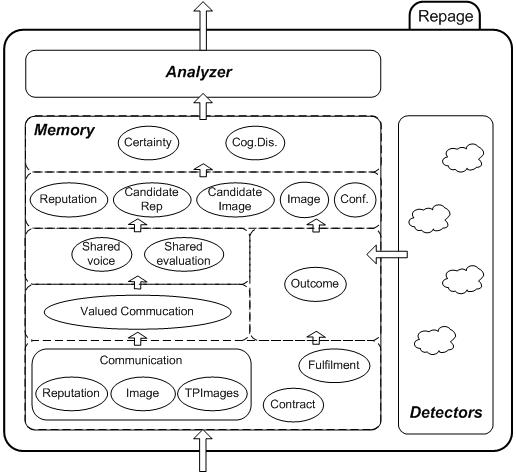
\includegraphics[width=\textwidth]{figures/repage.jpg}
	\caption{Repage architecture schematic (taken from \cite{Sabater2006})}
	\label{fig:Repage}
\end{figure}

At the first level of the abstraction hierarchy we have the basis of information to infer predicates, \textit{contracts}, \textit{fulfilments} and \textit{communication} (they are not themselves predicates, as no evaluation is attached). Contracts are agreements between two agents, while fulfilments are the results of the contract. Communication is the information about other agents that come from third parties. The second level is then constituted by inferences to an outcome, formed by a contract and its fulfilment, and valued information gathered from communications. This inferred predicates are not just tuples, they give an evaluation to the predicate, setting its belief strength. 

In the next level we have two predicates: \textit{shared voice} and \textit{shared evaluation}. The former is inferred from communicated reputation, and the latter from communicated images. 

The fourth level is composed from five types of predicates: \textit{Candidate Image}, \textit{Candidate Reputation}, \textit{Image}, \textit{Reputation} and \textit{Confirmation}. The candidate predicates are Images and Reputations that do not have enough support yet. Special detectors turns them to fill image/reputations when a strength threshold is surpassed. Confirmation is the feedback to a communication, received from comparing it to the image of the target. 

Finally the last abstractions level is composed of the predicates \textit{cognitive dissonance} and \textit{certainty}. Cognitive dissonance is a contradiction between relevant pieces of information that refer to the same target. This predicate may create instabilities in the mind of the individual, so the agent will most likely try to perform action in order to confirm the sources of this dissonance. Certainty represents full reliance on what the predicate asserts.

The last element is the analyser and its job is to propose actions in order to improve the accuracy of predicates in Repage and solve cognitive dissonances to produce certainty. The actions are proposed to the agent planner, leaving it to decide how to take this actions into account.

Image and Reputation are the predicates that provide a trust evaluation of a target, and as previously stated, they have a role, that represents two things: the agent actions that may affect to this evaluation, and a function that contextualizes the evaluative labels of \textit{VB, B, N, G, VG}. The probability distribution of the values gives out a picture of the target interaction forecast (e.g. a probability value of $0.5$ to VB gives a $50\%$ chance of the next interaction with the target being very bad).

The work described here is the only found that tries to establish an implementable architecture for a trust model, as most of the models created are purely theoretical. Furthermore, it fits to our goals of creating a trust assessment module, corresponding to the memory and detector components, and a trust decision module, corresponding to the analyser.


\subsubsection{BDI + Repage}
\label{subsubsec:Related work:Trust Models:BDI + Repage}
Pinyol \textit{et al.} \cite{Pinyol2009} proposes an integration of the Repage model, introduced in the previous Section \ref{subsubsec:Related work:Trust Models:Repage} into a BDI Agent\cite{Rao1995}. While the BDI model is not relevant to us, their work specifies \textit{BC}-logic, a belief first order logic that is capable of representing Repage predicate semantics and this is the part we will describe in the following paragraphs.

\textit{BC}-logic is structured hierarchically  


\subsubsection{Sutcliffe and Wang}
\label{subsubsec:Related work:Sutcliffe and Wang}
This work was published by Sucliffe and Wang in 2012\cite{Sutcliffe2012} and they built a trust model to figure out how cognitive social mechanisms emerge to follow Dunbar's \ac{SBH}\cite{Dunbar1998}, an evolutionary psychology theory that proposes that humans have a predisposition to build relationships in layers of decreasing intimacy. As trust has been acknowledged to be one of major component of human relationships, they demonstrate that simulating trust development and decay, through interactions and neglect, respectively, show the patterns predicted in \ac{SBH}.

From the model standpoint, its main interesting feature is that agents develop trusting relationships between one another, affecting interaction frequency between agents, by preferring to pick those with already high trust value. Additionally the trust relationship degrades as time passes by, with variable speeds depending on the current relationship level, giving stronger ties a slower descent. All in all, the model provides a good tool to simulate multi agent social behaviour, and may be interesting to predict trust degradation in the agent, albeit its described application for social simulations is a bit far from our scope.

\subsection{The Perception and Measurement of Human-Robot Trust}
\label{subsec:Related work:The Perception and Measurement of Human-Robot Trust}

Schaefer\cite{Schaefer2009} presents a trust perception scale providing a way of extracting an accurate trust score from humans interacting with robots. The scale is composed of 40 items that can be ranked from 0 to 100, in 10 point intervals. The final result it then averaged by adding all the item values and divided by the total number of items (40). 

While this work has been done specifically for \ac{HRI} we believe that a sub-set of this items can be used for the features used in the cognitive model of the user's trust, further described in Section \ref{subsec:Solution:Trust Assessment Module}. The items are listed in Table \ref{tbl:measurement.items.table} in appendix \ref{app:measurement.items.table}.
